\documentclass[a4paper]{article}

%% Language and font encodings
\usepackage[english]{babel}
\usepackage[utf8x]{inputenc}
\usepackage[T1]{fontenc}

%% Sets page size and margins
\usepackage[a4paper,top=3cm,bottom=2cm,left=3cm,right=3cm,marginparwidth=1.75cm]{geometry}

%% Useful packages
\usepackage{amsmath}
\usepackage{alltt}
\usepackage{graphicx}
\usepackage[colorinlistoftodos]{todonotes}

\title{A Progressive Web App (PWA)-based Mobile Wallet for Bazo}
\author{Jan von der Assen}

\begin{document}
\maketitle

\begin{abstract}
  Your abstract.
\end{abstract}
\newpage
\tableofcontents
\newpage


\section{Introduction}
%% Importance etc of Blockchain based currencies

A financial service provider based in Zurich developed a bonus program that incentivizes customers to use its credit and debit cards. With every purchase with this card, customers collect virtual points. Several industry partners are participants of this bonus program. The virtual points collected can be exchanged for gift cards form partners registered via the Web site or an app. The way that these services can be used in the traditional system puts the company into a central role, thus requiring administrative efforts to enable both customers and partners to exchange virtual points. In order to decentralize the financial service providers position a blockchain based currency, Bazo (Esperanto: base; foundation), was developed at the University of Zurich. The intention of the currency is to map virtual points to coins in the crypto currency.
The focus of this thesis lies on the implementation and evaluation of a Mobile Wallet for said currency. Features as well as requirement and implementation details are gathered during the project in an explorative way in partnership with the company.
\subsection{Motivation}
Traditional payment systems require a centralized institution in order to maintain a currency and support operations such as issueing, transferring and determining state of currency units. Centralizing the issuer of the virtual coins for each operation that can be performed on the virtual currency further prohibits the direct trading of virtual points between users.
In the case of the partner company this resulted in a limited awareness and usage of the incentivization program by customers as well as partners.
With the new cryptocurrency developed at the University of Zurich which is tailored to the requirements of a financial service provider, it is possible to still maintain control over the currency since the company remains in an issuer position. In order to let end users such as customers and partners interact with the currency as well as making the program more transparent, further development efforts are taken. This should pose a first complete prototype of a currency ecosystem where the financial service provider can evaluate the new solution with real costumers and gain insight on how blockchain technologies can be used to improve certain processes. This involves the development of a Wallet to let users trade Bazo coins as well as to improve the payment process since smartphone capabilites can be used to transfer payment information from device to device.

\subsection{Description of Work}
This thesis covers the design, implementation, and evaluation of a mobile wallet for the Bazo cryptocurrency. In order to run the client as trustless as possible, a light client implementation needs to be integrated to the Bazo wallet. This involves the integration and development of interfaces to enable -this-.
The development should leverage existing resources from similar projects where a Mobile Wallet was implemented.
It is required to find a way to transmit payment information with native elements such as NFC and Bluetooth. However, a fallback solution needs to be implemented to allow a broad range of users to participate in the program.
In order to support the complete use case for customers and partners, it is required to integrate -third party- services from the service provider.
The application needs to be tested in a pilot project where the Bazo cryptocurrency is used for payment. 




\subsection{Outline}
The main section of the report is structered as follows:
In chapter 2 an introduction to leveraged technologies, the traditional and envisioned transaction process is given. Further, related work  as well as other activities in the project are introduced. Chapter 3 focuses on the design of a Mobile Wallet that satisfies the supplied requirements. The concrete implementation of the design is explained in chapter 4. In chapter 5 the prototype and the findings from developing the Wallet are evaluated and the results compared.
Chapter 6 summarizes and concludes the report.
\newpage

\section{Background and Related Work}
\subsection{Background}
\subsubsection{Cryptocurrencies}
\subsubsection{Web based Wallets}
\subsubsection{Progressive Web Applications}
\subsubsection{Traditional payment process}
In the traditional process, customers were incentivized to use debit and credit cards issued by the company by rewarding the customer with points of a virtual currency based on the transaction volumes.
Through contracts that are established between the company and partner companys, the company can trade the customers virtual points against gift cards from partner companys.
Based on the terms established in the contract, the partner companies are disbursed for the value of the gift cards, which customers can redeem at the partner company.
Similar to the process of exchanging virtual points for goods, the company also has to act as a middleman when users want to exchange their points amongst each other. Both these cases pose a significant administrative effort for the company. Further disadvantages are the limited transparency of the program to users and that the virtual points have a relative short lifecycle.

\subsubsection{Envisioned payment process}
The envisioned system is supposed to overcome the stated disadvantages, by mapping the virtual points to a currency that can be used directly to make transactions between users or between user and partner company.
The financial company rewarding with the virtual points should still remain in a central position for the currency and control aspects such as issueing new units and accounts.
The Wallet that is developed for making transactions with the currency is required to support user to user transactions as well as transactions between a user and the merchant. This implies that there is a way that both merchants and users can request money by supplying payment information in a device to device manner. Since merchants may have more advanced payment system, a possibility to integrate third party interfaces into the payment process is required. The actual requirements and design of how transaction information can be transferred needed to be explored with the company and is further described in chapter \ref{fig:tps}.


\subsection{Related Work}
\subsubsection{Bazo}
Bazo is a cryptocurrency developed at the CSG at the University of Zurich. The currency was tailored to the use case of the financial service provider, which acts as a central institution that is able to create new coins and accounts. This makes the currency private, since an invite needs to be used to use the currency. This differs from various popular cryptocurrencies such as Bitcoin and Ethereum [xy] which are both open to the public. Similar to the approach taken in Ethereum, Bazo implements an account-based data model. Consensus in the Bazo network is achieved through a Proof of Work algorithm, although there are drawbacks from employing this strategy. More information about the current state of research of the consensus protocol in Bazo can be found in \ref{Bazo Block Explorer}.

\subsubsection{Bazo Client Implementations}
\subsubsection{Coinblesk}
\subsubsection{Bazo Block Explorer}
\newpage


\section{Design}

\subsection{Application Structure}

\subsubsection{Progressive Web Applications}
\subsubsection{Network Communication}
\subsubsection{Interfaces}

\subsection{Transaction Information}
One requirement, that is that Bazo coins can be exchanged between users without direct involvement or administration from the service provider was incorporated into the core design of the Bazo currency. To fulfill said requirement it is vital that transaction informations can be shared between users of the Bazo Wallet. This section outlines how transaction information can be shared with the Bazo Wallet.
%Search for papers, resources etc.
Sharing transaction information in native applications is often achieved with technologies such as NFC, Bluetooth or by encoding and reading transaction information from a Quick-Response Code.
\subsubsection{Schema}
In order to communicate Bazo Transactions to other devices and applications, an URI Scheme was designed to hold transaction information, so that a requesting party can communicate it. The grammar and structure for the schema followed the \cite{bip21} 21st Bitcoin Improvement Proposal for an URI scheme since it contained all necessary elements to fulfill the requirement. The URI Schema consists of a required part which holds the protocol name and the recipient's fully qualified bazo address.


\[
\underbrace{\overbrace{bazo:}^{\mathrm{protocol}}\overbrace{MIGfMA0GCSqGSIb3DQEBAQUAA4GNADC}^{\mathrm{bazo address}}}_{\mathrm{required components}}
\underbrace{\overbrace{?amount=123}^{\mathrm{amoun t}}\overbrace{?label=1 Coffee}^{\mathrm{label}}\overbrace{?message=Message}^{\mathrm{message}}}_{\mathrm{optional components}}
\]


% reference nfc bridge
This implies, that the Bazo Wallet and other applications that need to interact with it need to be able to encode and decode transaction information as supplied in the described grammar.
For the web-based wallet this transaction info should also be an optional parameter of the URL of the payment page. This allows that a complete URI to the payment page with all required transaction information can be shared among users or between merchants and users.
This enables to encode complete transaction information as well as a an URI to the application page with the transaction information into media such as a QR-Code. This has the benefit, that all users of the Wallet can exchange payment information without having to know about the Schema.
Since merchants frequently have more advanced payment systems and don't want to encode payment information into media such as QR-Codes for each new transaction, the payment page of the Wallet also needs to be able to accept additional parameters, by which the Wallet can then query the transaction amount from a service.
The schema below shows the URI endpoint of the payment page, together with additional parameters that can be supplied to have the payment page prefilled with transaction information. This procedure is further described in Figure\ref{fig:POS}.
\[
\underbrace{\overbrace{https://host/:}^{\mathrm{Host}}\overbrace{/auth/user/send}^{\mathrm{payment page}}}_{\mathrm{required components}}
\underbrace{\overbrace{posid=323}^{\mathrm{POS identification}}\overbrace{?paymentinfo=bazo://123123}^{\mathrm{transaction info}}}_{\mathrm{optional components}}
\]

The implementation of the module to encode and decode bazo encoded transaction information is described in \ref{xy}.
%reference impl

\subsubsection{Device Sharing}
In order to explore further possibilities on how to extend the browser support for native API's a Proof of Concept was implemented. The PoC was targeted to the android Platform, since NFC support is still fairly limited on iOS devices at the time of the design. The PoC, further referenced as 'NFC Bridge', should run as a background service and enable two processes.
\begin{enumerate}
\item Reading NFC devices:
The application should be registered as a handler for NFC messages. If an NFC message is read from another NFC device such as another active device or an NFC Tag, the user is prompted with applications that can handle the data format. If the user selects the NFC Bridge application, the data received from the NFC Adapter should be parsed and the user prompted with the Payment page of the Bazo Wallet. The payment page is then prefilled with the payment information extracted from the NDEF message.
\item Pushing to NFC devices: The NFC Bridge application should allow the PWA-based Bazo Wallet to push handover encoded transaction information which can then be pushed to NFC devices and tags.
The first design sketch included that communication between the Bridge application and the Bazo Wallet is done through an HTTP or Websocket. This implied that the NFC Bridge is running as a background service, listening for NFC messages and keeping the server alive.
Since the android platform allows starting the application when an NFC message is received through the configuration of application intents, this design was preferred.
\end{enumerate}

\subsubsection{Merchant options}\label{fig:tps}
In order to completely support the payment process, which does require interaction of the application with backend services from the financial service provider, interfaces need to be integrated into the application.
This is also necessary since some platform do not support WebNFC in the browser, which means that the payment process can not be carried out in a complete device-to-device manner. On iOS devices support for NFC access is restricted to native API's and the functionality is limited to reading passive NFC Tags.
In order to get the complete payment process depicted, the payment process that is to be developed can be described as follows. The user of an iOS device can use his any NFC Tag Reader app from the app store. Before the payment process can be started, the merchant needs to supply payment information in form of a correct bazo address as well as some token that represents the Point-of-sale system. The merchant should have the possibility to write these informations to the NFC Tag at the POS, using the Mobile Wallet application.
Once this set up is in place, the user will approach the POS System and may start the payment process. The cashier will scan the items, and the POS System will automatically associate the POS ID with the transaction amount. The user can now use any existing iOS or android application to read the NFC tag. Since both payment and transaction information is encoded in a URL, the user is taken to the payment page of the Mobile Wallet, where the POS ID is used to query the transaction amount from the POS System. Since the Bazo Address is supplied in the URL as well, the user can confirm the payment. Once confirmed the Mobile Wallet will sign the transaction and send it into the Bazo network. Figure
\ref{fig:POS} shows the process of transferring transaction information and transaction issueing under the constraint that a third party service needs to be queried.

\begin{figure}
\centering
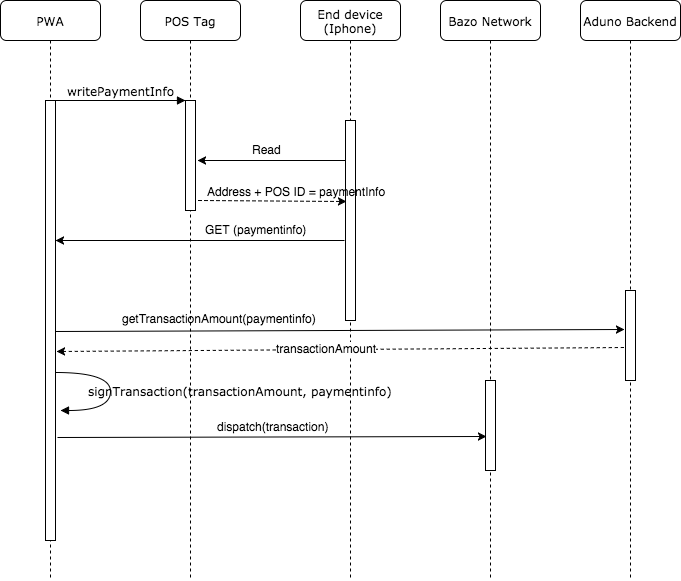
\includegraphics[width=1\textwidth]{diagrams/POS_flow.png}
\caption{\label{fig:POS}The application flow of transferring payment information.}
\end{figure}

\subsection{Communication}
%% Interfaces includes integration of existing services
\subsubsection{Bazo Interfaces}
\subsubsection{Payment System Interfaces}

\subsubsection{Security Considerations}

\newpage

\section{Implementation}
\subsection{Architecture}
\subsubsection{User Interface}
\subsubsection{Storage}
\subsubsection{State}
\subsubsection{Network Handling and Communication}

\subsection{Transaction Sharing}
\subsubsection{Web APIs and Browser Support}
\subsubsection{NFC}

\subsubsection{Bluetooth Low Energy}
\subsubsection{Quick Response Codes}
\subsubsection{Fallback Solutions}
\subsubsection{Transaction Encoding}

\subsection{Blockchain Interaction}
\subsubsection{Bazo Client}
\subsubsection{Client Integration}
\subsubsection{Transaction Signing}
\subsubsection{Data Queries}

\subsection{Testing}
\newpage

\section{Evaluation}
\subsection{Prototype Evaluation}
\subsection{Comparison}
\subsection{Limitations}
\subsection{Future Development}
\subsection{Future Work}
\newpage

\section{Summary and Conclusions}
An introduction citing \cite{Liviosgier}

\newpage

\bibliographystyle{alpha}
\bibliography{sample}

\end{document}
